\chapter{Lyman-\texorpdfstring{$\alpha$}{a} Histories of Massive Halos}

\section{A Morphological Introduction}

In Figures \ref{fig:rogues1}, \ref{fig:rogues2}, \ref{fig:rogues4}, and \ref{fig:rogues8} we present surface brightness images for nearly half of all the snapshots that were used in this work. \red{is adding a colorbar a difficult implementation?  [no big deal if it is since you put the scale in the caption]}
From just a bye-eye analysis of these images, we can notice a few trends, some of which will become relevant later on in this work.
There is definitely some redshift evolution of these objects, but there appears to be a different behavior between halos A1 and A2 as compared to A4 and A8.
In halos A1 and A2, the physical extent of the Ly$\alpha$ surface brightness does not seem to evolve much with redshift, whereas in A4 and A8 there seems to be monotonic growth over redshift.
Additionally, while halos A4 and A8 become brighter and more extended around $z=2$, halo A2 appears to be more compact at low redshift, possibly indicating some evolution out of a blob phase of galaxy evolution.
In this work we only analyze snapshots down to $z=2$, so we are unable to comment in detail on the appearance of these objects at low redshift, but do note that LABs have been detected at low redshift \citep{Barger2012,Prescott2013} so it would not be particularly surprising for a halo to still be in a blob-like phase at $z=2$, even though most have been observed at $z\sim3$.

We also present Figures \ref{fig:A4stars} and \ref{fig:A4gas} to provide some insight into the distribution of stars and gas that correlate to our largest and brightest halo.
The primary insight from these figures is that while Ly$\alpha$ approximately tracks the presence of gas, it is much more spatially dispersed.
Additionally, by visualizing directly the presence of gas and stars we can see that these massive halos undergo numerous mergers over thier formation history.
It is unclear whether one can connect mergers to the formation of Ly$\alpha$ blobs; it appears that these merger events serve to disrupt what might be a smaller and possibly disky structure in the central galaxy.
But we do not really have the necessary tools test this theory that major mergers are required to produce the spatially extended Ly$\alpha$ surface brightness, since it is the nature of these high-mass galaxies that they undergo a large number of mergers.
That is, while one could construct an isolated high-mass halo or galaxy that system would be non-physical so it is unclear what insight could be derived from its behavior.

\begin{figure*}
    \centering
    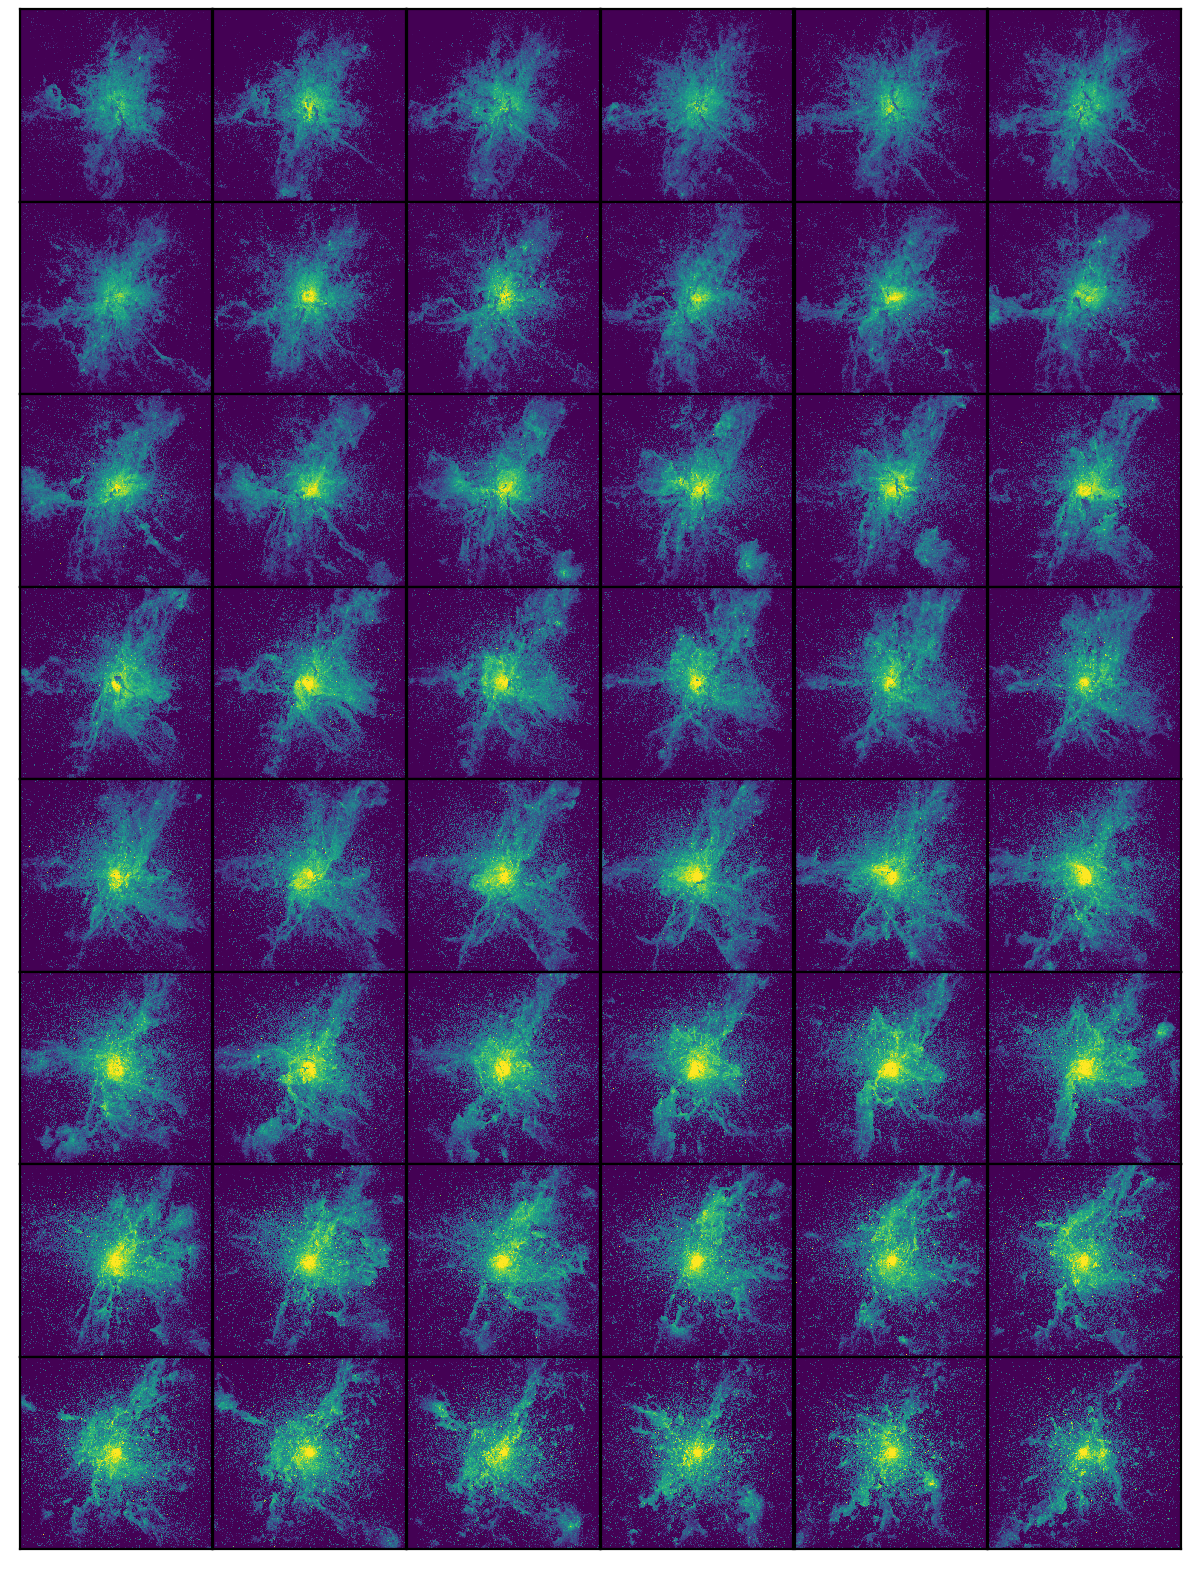
\includegraphics[width=\textwidth,keepaspectratio]{figures/rogues_A1.png}
    \caption{
        Ly$\alpha$ surface brightness images of of halo A1 from $z=4.5$ (top-left) to $z=2.0$ (bottom-right).
        All images are 75$\times$75 physical kpc across, and are scaled from $2\times 10^{-19}-10^{-16}\ \rm{erg}\ \rm{s}^{-1}\ \rm{cm}^{-2}\ \rm{arcsec}^{-2}$.
    }
  \label{fig:rogues1}
\end{figure*}

\begin{figure*}
    \centering
    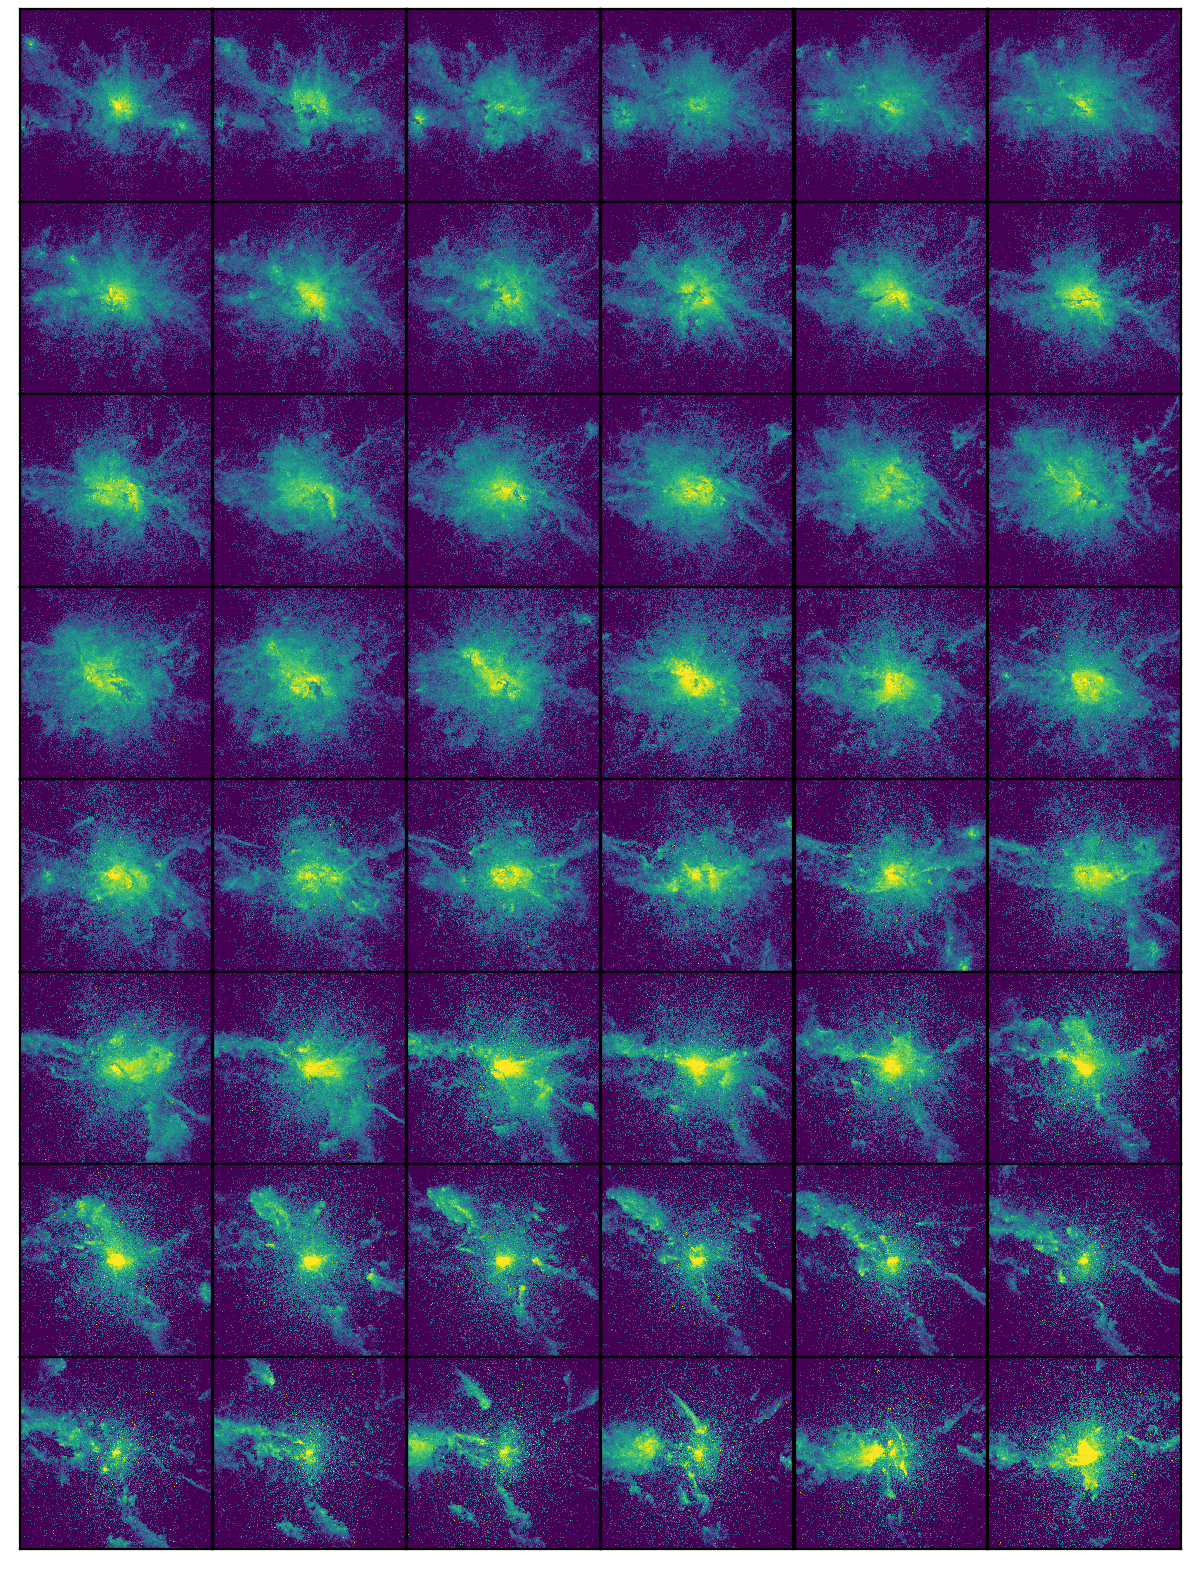
\includegraphics[width=\textwidth,keepaspectratio]{figures/rogues_A2.png}
    \caption{
        Ly$\alpha$ surface brightness images of of halo A2 from $z=4.5$ (top-left) to $z=2.0$ (bottom-right).
        All images are 75$\times$75 physical kpc across, and are scaled from $2\times 10^{-19}-10^{-16}\ \rm{erg}\ \rm{s}^{-1}\ \rm{cm}^{-2}\ \rm{arcsec}^{-2}$.
    }
  \label{fig:rogues2}
\end{figure*}

\begin{figure*}
    \centering
    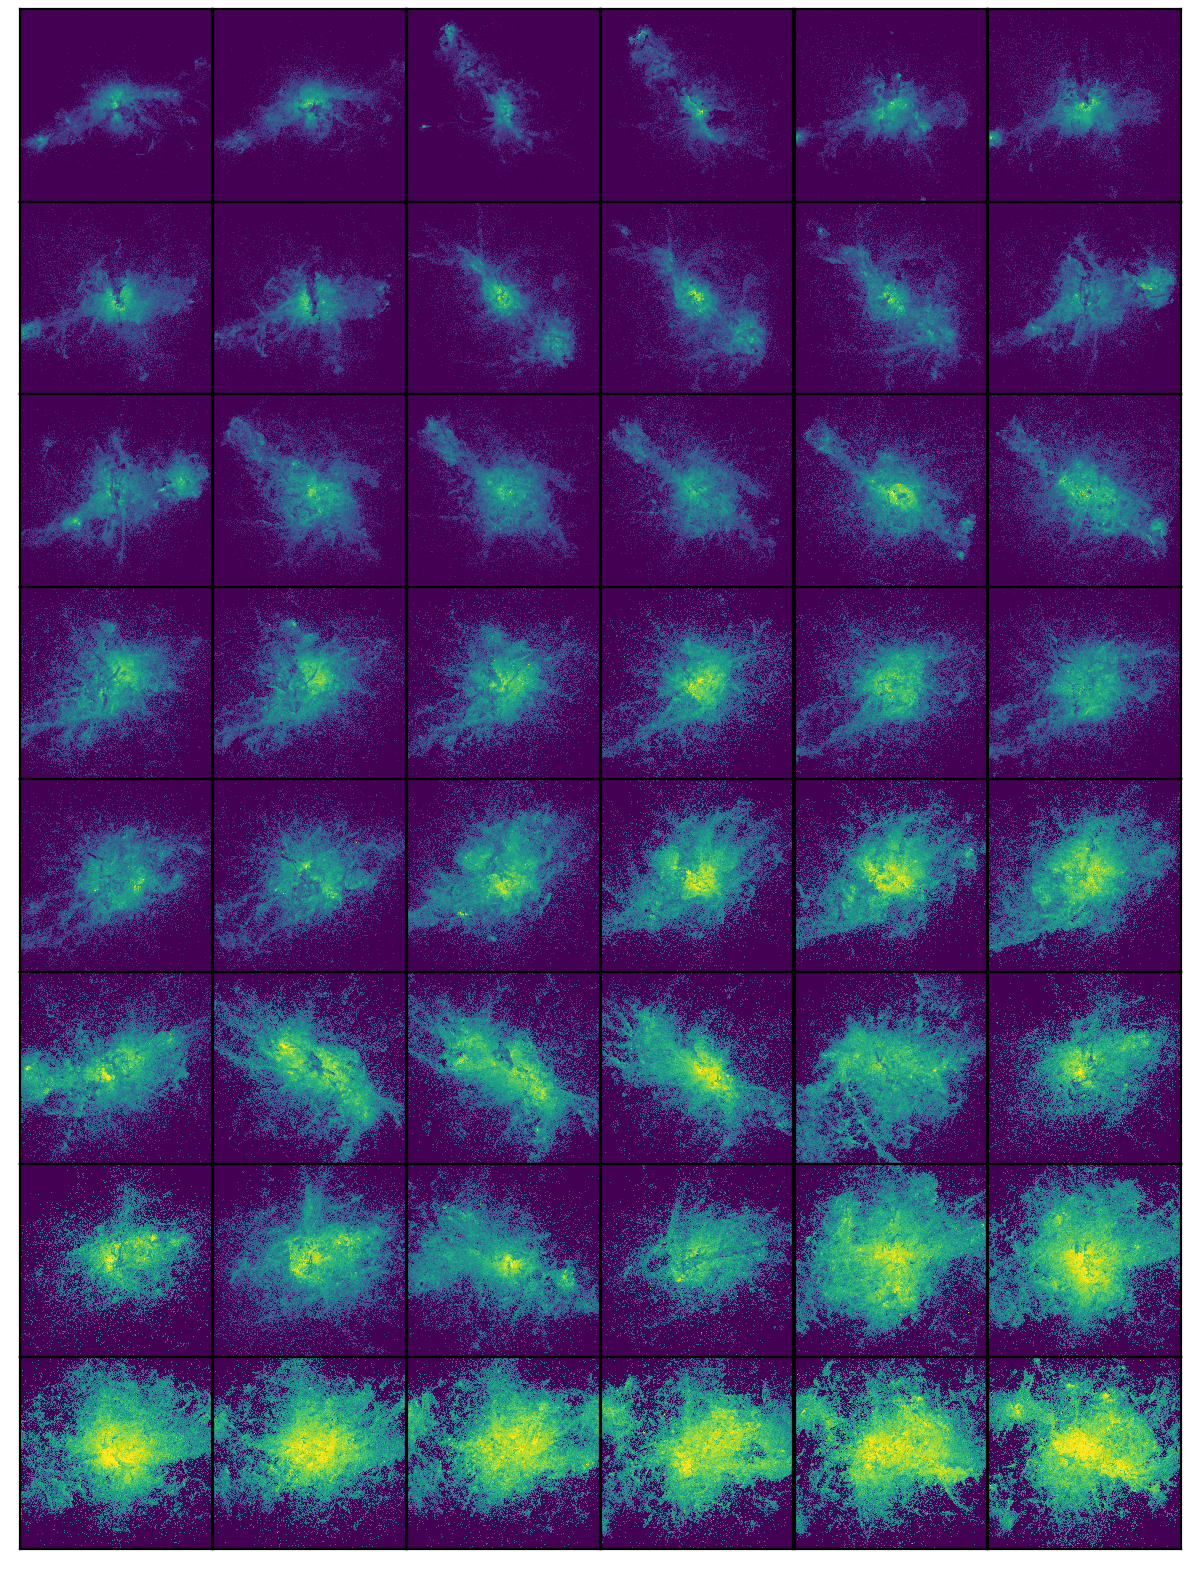
\includegraphics[width=\textwidth,keepaspectratio]{figures/rogues_A8.png}
    \caption{
        Ly$\alpha$ surface brightness images of of halo A8 from $z=4.5$ (top-left) to $z=2.0$ (bottom-right).
        All images are 75$\times$75 physical kpc across, and are scaled from $2\times10^{-19}-10^{-16}\ \rm{erg}\ \rm{s}^{-1}\ \rm{cm}^{-2}\ \rm{arcsec}^{-2}$.
    }
  \label{fig:rogues8}
\end{figure*}

\begin{figure*}
    \centering
    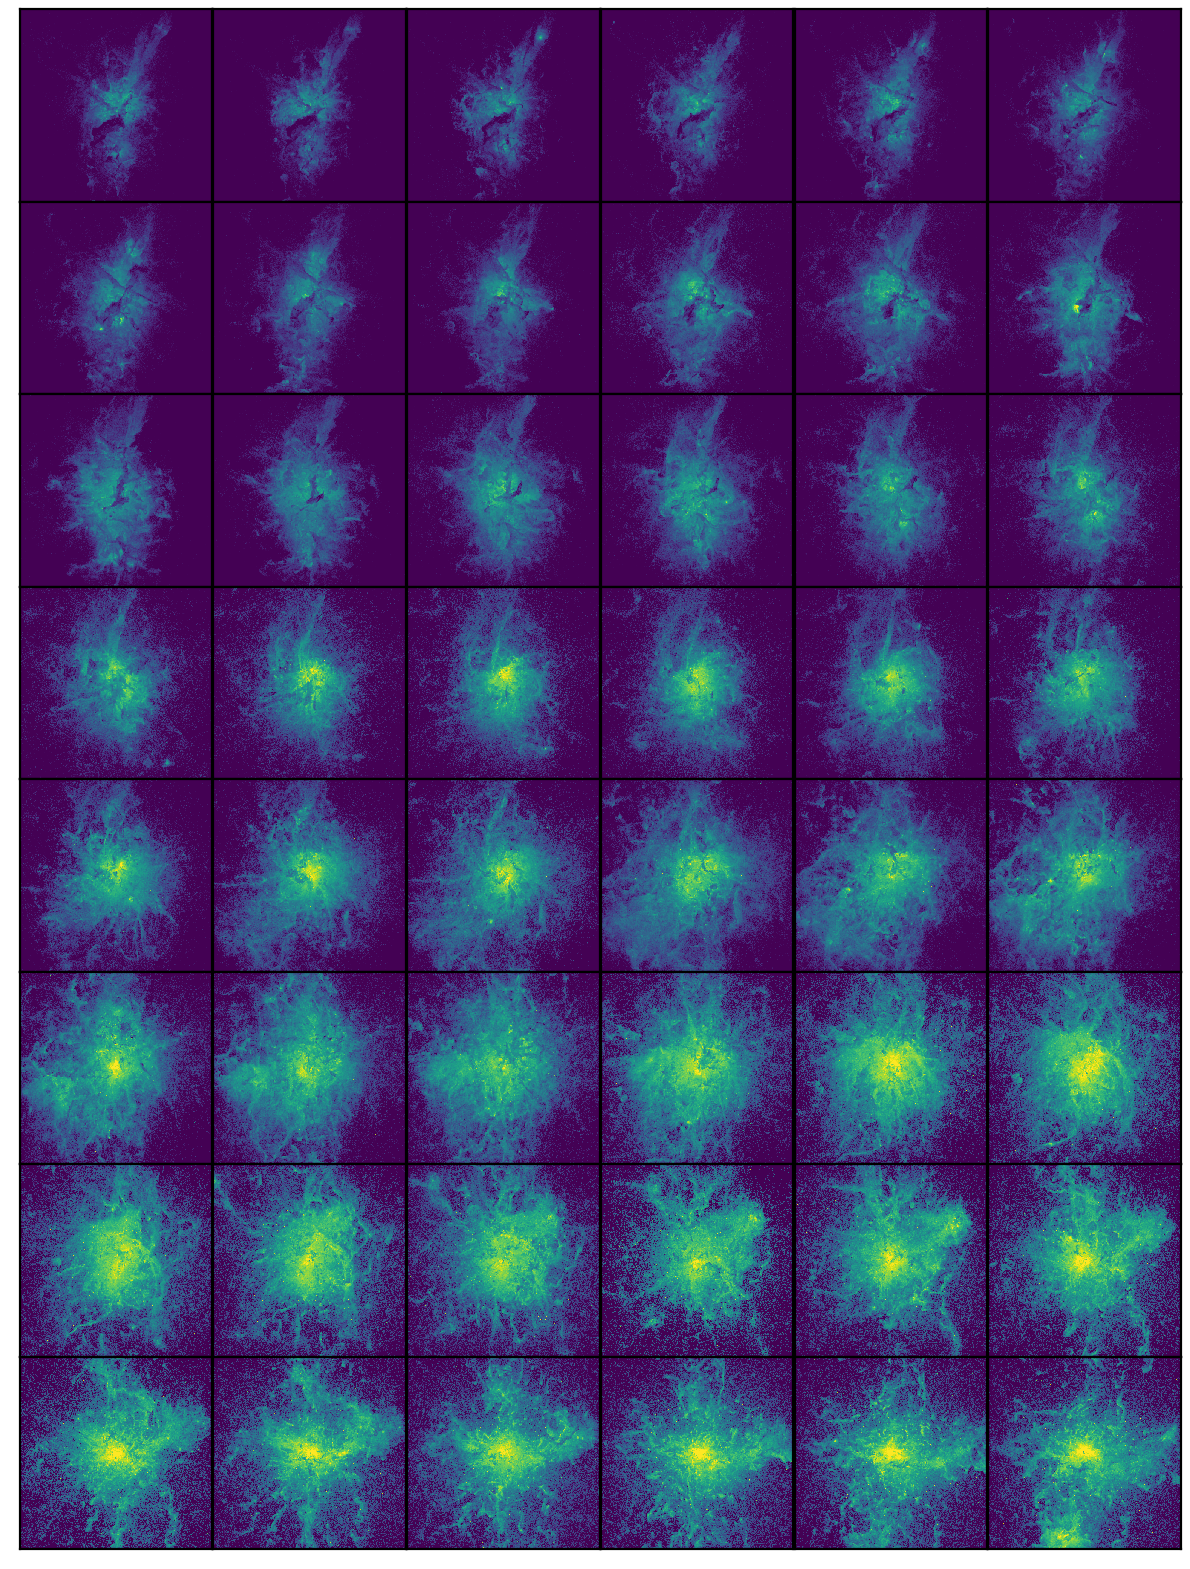
\includegraphics[width=\textwidth,keepaspectratio]{figures/rogues_A4.png}
    \caption{
        Ly$\alpha$ surface brightness images of of halo A4 from $z=4.5$ (top-left) to $z=2.0$ (bottom-right).
        All images are 75$\times$75 physical kpc across, and are scaled from $2\times10^{-19}-10^{-16}\ \rm{erg}\ \rm{s}^{-1}\ \rm{cm}^{-2}\ \rm{arcsec}^{-2}$.
    }
  \label{fig:rogues4}
\end{figure*}

\begin{figure*}
    \centering
    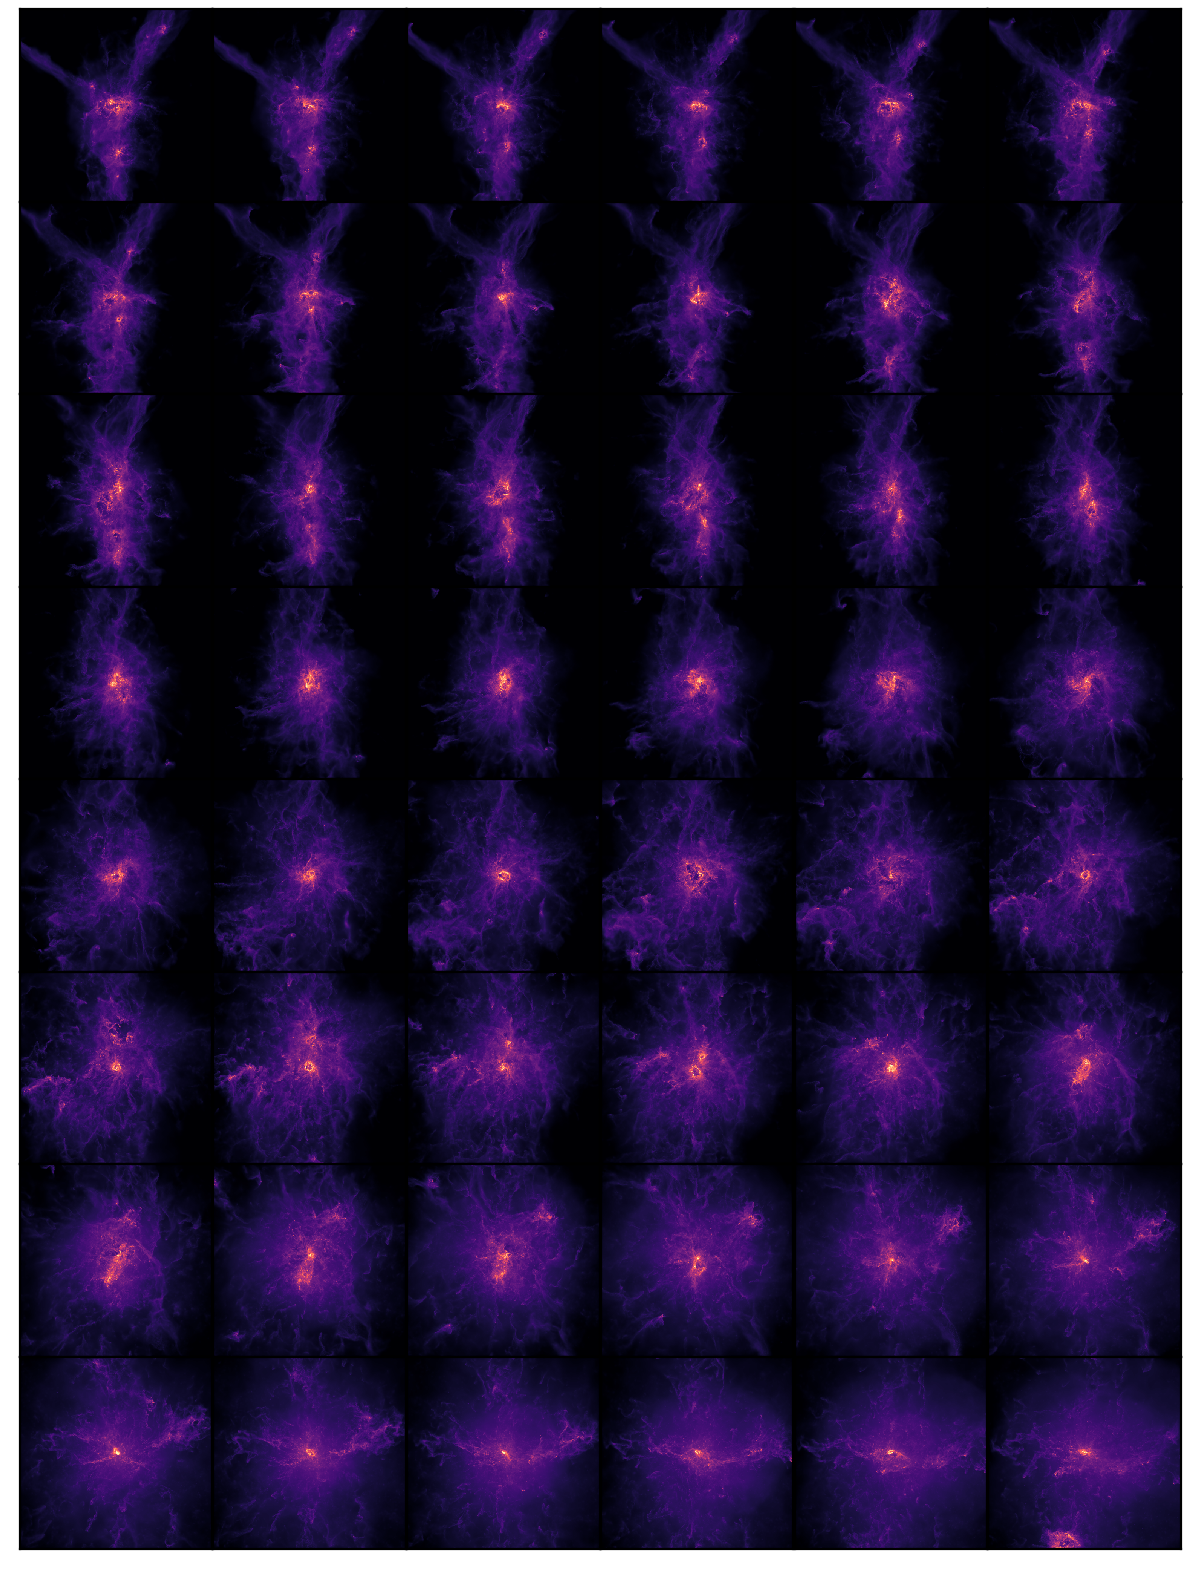
\includegraphics[width=\textwidth,keepaspectratio]{figures/rogues_gas.png}
    \caption{
        Gas surface density of halo A4 from $z=4.5$ (top-left) to $z=2.0$ (bottom-right).
        All images are 75$\times$75 physical kpc across, and are scaled from $2\times10^{-4}-2\times10^{1}\ \rm{g}\ \rm{cm}^{-2}$.
    }
  \label{fig:A4gas}
\end{figure*}

\begin{figure*}
    \centering
    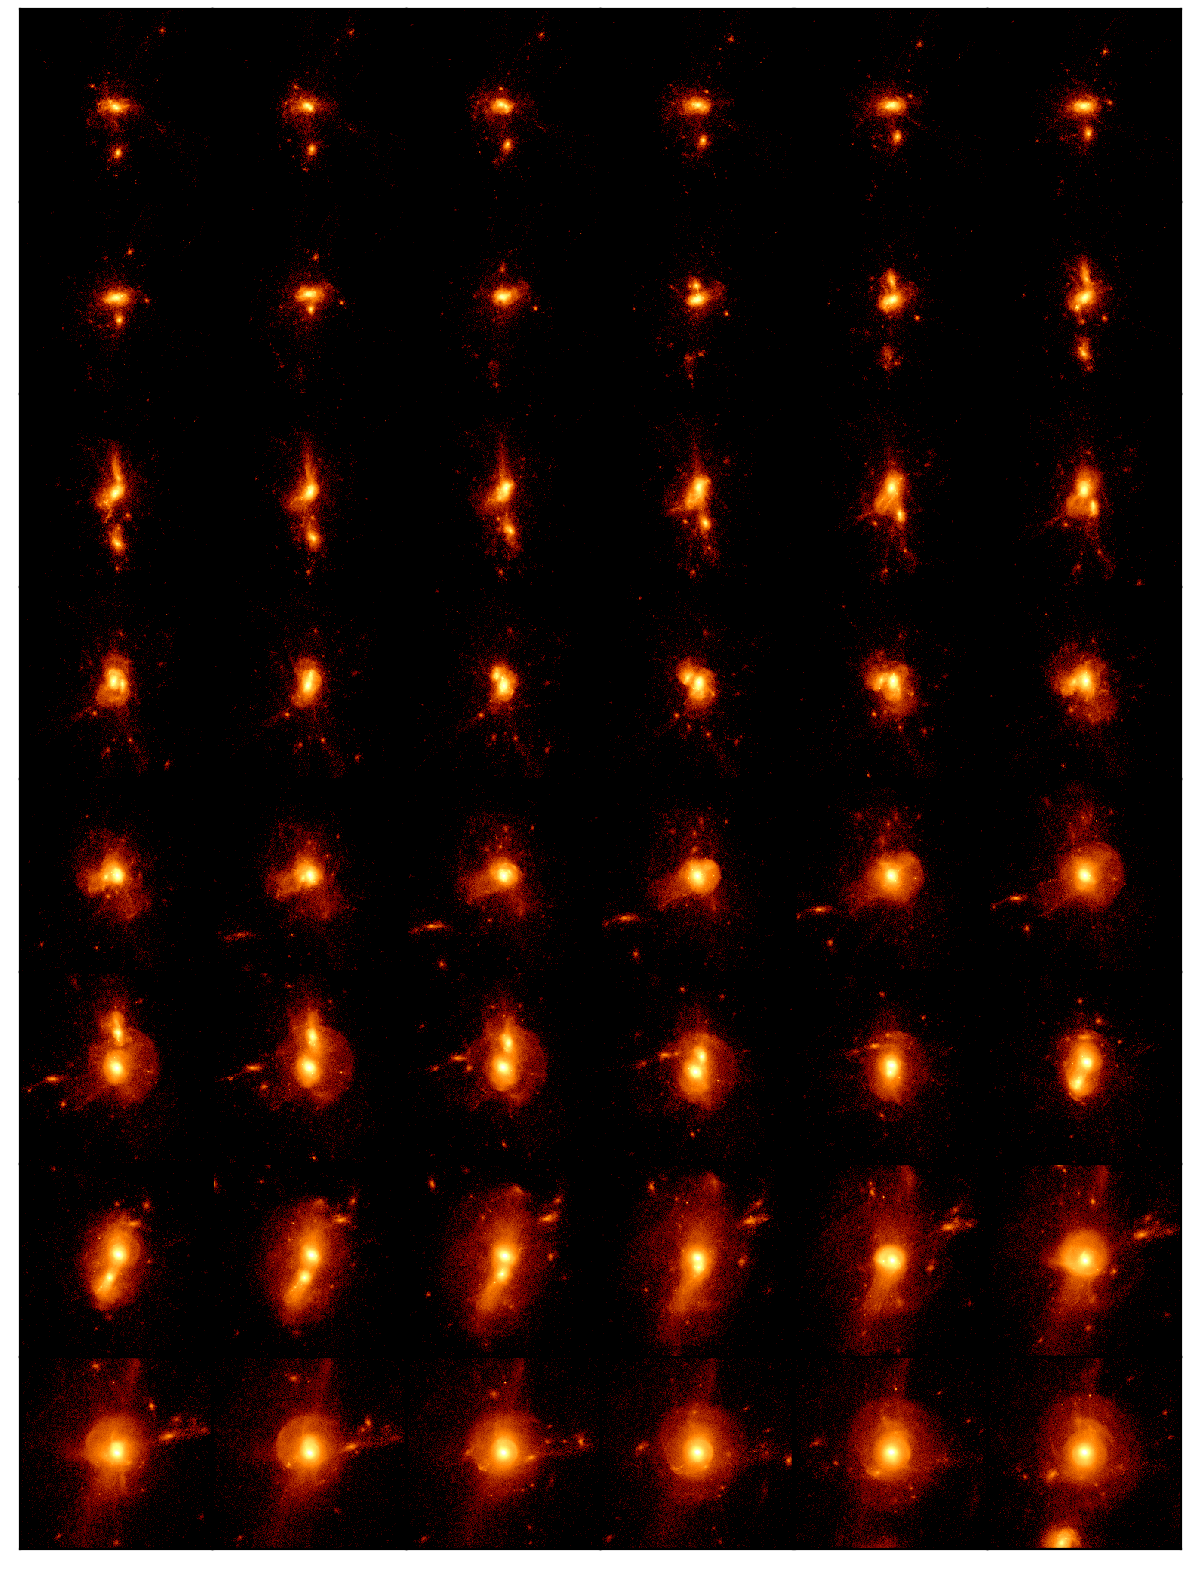
\includegraphics[width=\textwidth,keepaspectratio]{figures/rogues_stars.png}
    \caption{
        Gas surface density of halo A4 from $z=4.5$ (top-left) to $z=2.0$ (bottom-right).
        All images are 75$\times$75 physical kpc across, and are scaled from $10^{4}-10^{9}\ \rm{M}_{\odot}\ \rm{kpc}^{-2}$.
    }
  \label{fig:A4stars}
\end{figure*}



\section{The formation of Ly\texorpdfstring{$\alpha$}{a} blobs}
\label{sec:formation_of_labs}

% Rogues gallery with gas and stars?

First we need to establish that our simulations actually form Ly$\alpha$ blobs.
As mentioned in \S~\ref{sec:blob_definition}, there is neither a formal definition for a LAB, nor does there appear to be any consensus in the literature on an informal definition.
Therefore, we explore two informative criteria for objects classified as Ly$\alpha$ blobs and compare those to our simulations: total Ly$\alpha$ luminosity and spatial extent.

We first consider the Ly$\alpha$ luminosity component of a blob definition.
In Figure~\ref{fig:luminosity_redshift}, we plot the Ly$\alpha$ luminosity for our model galaxies as a function of time from $z\approx5-2$.
For comparison, we also show the Ly$\alpha$ luminosities for a number of observed LABs mentioned in Table \ref{table:labs}.
The Ly$\alpha$ luminosity of our model galaxies varies substantially, but broadly overlap  with the observed range of luminosities over the considered redshift range.

\begin{figure}
    \centering
    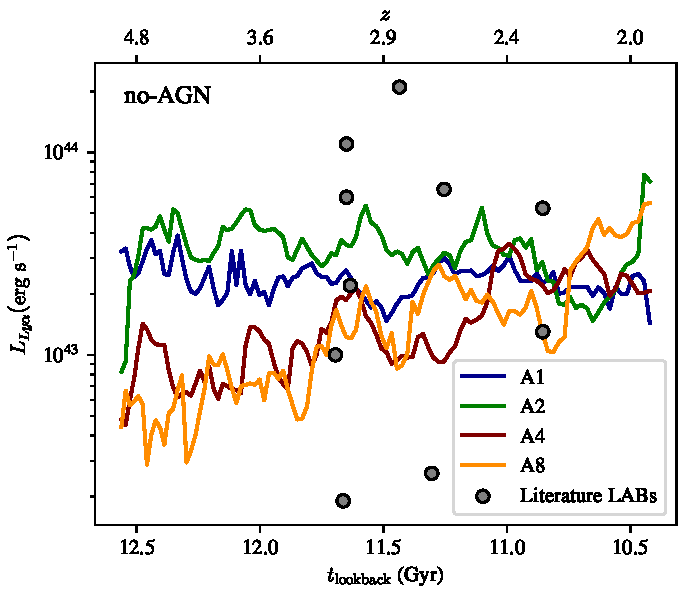
\includegraphics[width=\textwidth,height=\textheight,keepaspectratio]{figures/luminosity_redshift.pdf}
    \caption{
        Ly$\alpha$ luminosity for a median line of sight for each galaxy in our sample of MassiveFIRE (lines), with observational data from Table~\ref{table:labs} overplotted as points.
        Broadly, our LABs fall within the range of observed objects between z=5 and z=2.
    }
    \label{fig:luminosity_redshift}
\end{figure}

Even here in such a simple plot, there is subtelty.
The model for LABs we present here does not include the effect of AGN in any sense, and it is well-accepted that AGN have an important role in galaxy formation.
Additionally, we are presenting the luminosity of these objects along a median line of sight.
This is primarily chosen to simplify the visualization and because it gives the right impression, which is that these objects are typically bright enough to be called a LAB.
We will return to this subject repeatedly: Line of sight matters.
Finally, note that all these objects display different redshift evolution.
A4's luminosity increases over time, while A1 and A2 are approximately constant or decreasing.
Given $n=4$ it's not really possible to pick a representative object, each of these objects behave differently which we will elaborate on as we discuss the mechanisms of emission in more detail.

The second component to our LAB definition is spatial extent.
Some studies employ surface brightness profiles to characterize the spatial extent of objects \citep[e.g.][]{Wisotzki2018, Steidel2011}.
However, as we will demonstrate, the blob morphologies are sufficiently disordered and asymmetric that it is reasonable to call into question the meaning of a radial profile.
Specifically, the problem is that to define a surface brightness profile one needs to identify a center.
This is not a problem for some systems, but the LABs we are studying form around/from high-mass galaxies, and such systems undergo major mergers very often.
This has a dual effect; at many times these systems do not have a clear center, or they have two bright central regions, or they have two bright central regions at some lines of sight and not at others.
In addition to the lack of a center LABs tend to form from systems that are just asymmetrical.
The challenge of data visualization and communication in this case is to collapse a 2d image into a 1d line so that we can display multiple objects at the same time for easy comparison in the 2d medium that we are so accustomed to.
Therefore, we choose axes for this plot in an attempt to not produce any incorrect impressions about symmetry.
To characterize blobs by their surface brightness, in Figure~\ref{fig:area_plot}, we plot the area enclosed by a number of isophotes as a function of the isophotal luminosity.
We also attempt to compare these to known LABs (from Table \ref{table:labs}).
Since we want to plot an area and most publications only mention a radius or semi-major axis of a blob, we assume such blobs are circular to deduce an area, and therefore denote these as upper limits since this ``radius'' is most likely the largest radius of the blob, not the radius of circle with equivalent area.

As is evident from Figures~\ref{fig:luminosity_redshift} and ~\ref{fig:area_plot}, our model galaxies display reasonable Ly$\alpha$ luminosities and enclosed areas as a function of limiting surface brightness when compared to observations.
In Figure~\ref{fig:MUSE}, we take a $z \sim 2$ snapshot of our fiducial model and convolve the model Ly$\alpha$ surface brightness with the MUSE point source function.

We will spend the next few sections unpacking Figures~\ref{fig:luminosity_redshift} and \ref{fig:area_plot}, exploring {\it why} these galaxies emit copious Ly$\alpha$ emission.

\begin{figure}
    \centering
    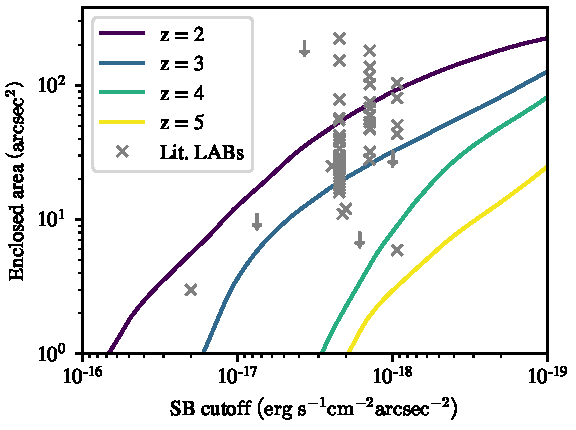
\includegraphics[width=\textwidth,height=\textheight,keepaspectratio]{figures/area_profile.pdf}
    \caption{
        Comparison of blob sizes in our models to literature sizes.
        We define the size as the area enclosed with in a surface brightness contour, and plot against units in an attempt to be consistent with the units used by a majority of published observations.
        Our contours pass through the space covered by observations, which is strong evidence that we are reproducing the observed spatial extent of these objects.
    }
  \label{fig:area_plot}
\end{figure}

\begin{figure*}
    \centering
    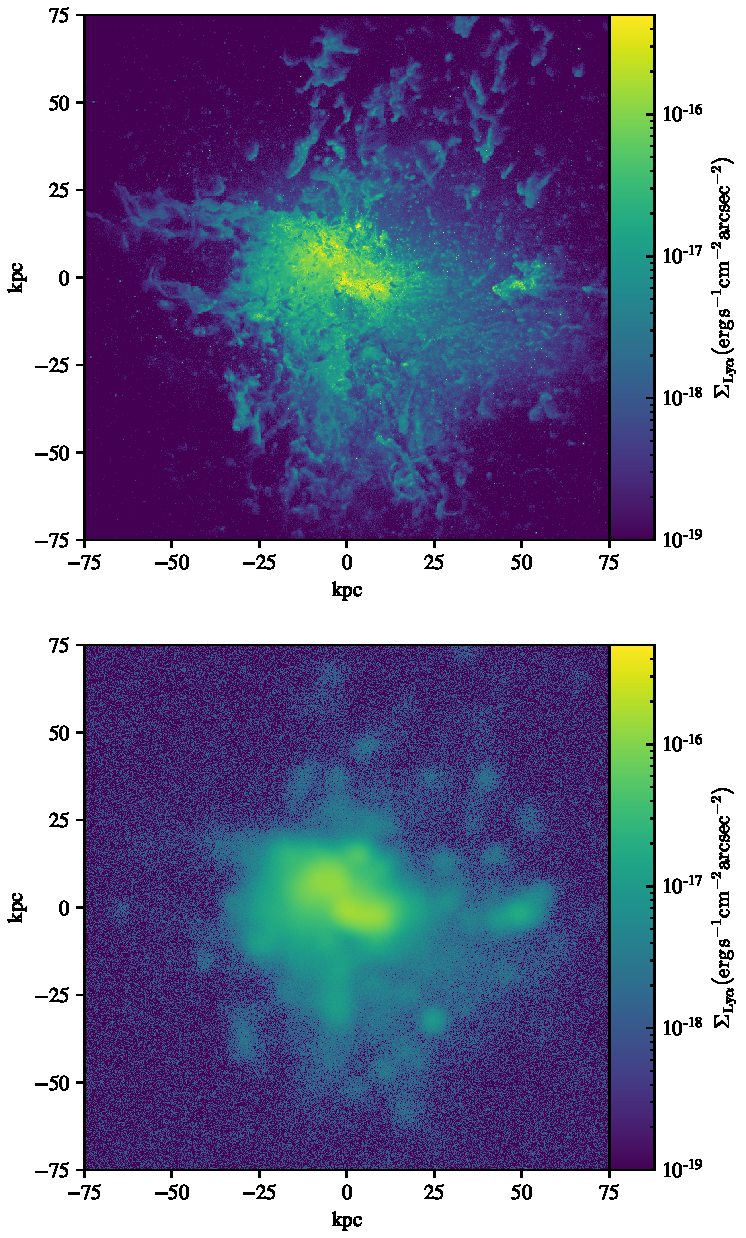
\includegraphics[width=\textwidth,height=0.85\textheight,keepaspectratio]{figures/muse_comparison.pdf}
    \caption{
        At left, we show one of our surface brightness images at a very high resolution, and at right we convolve the surface brightness down to the resolution of MUSE with Gaussian noise at $\sigma=10^{-18}$ erg/s to produce an image that more closely resembles current observations of LABs.
        The surface brightness image here is generated with $10^{9}$ MCRT samples, and so it is of considerably higher quality than our typical simulations.
    }
    \label{fig:MUSE}
\end{figure*}


\section{Origins of Observed Ly\texorpdfstring{$\alpha$}{a} Photons in Giant Blobs}
\label{sec:origins}

In this section, we conduct a series of numerical experiments in order to characterize the driving sources of Ly$\alpha$ radiation from our model blobs.
We investigate the relative contributions of emission from gas cooling and recombinations (Figure~\ref{fig:recombination_collision}, Figure~\ref{fig:agn_recombination_collision}), the impact of the ionizing UV background (Figure~\ref{fig:uvb_morphology}), and the presence of AGN (Figure~\ref{fig:agn_comparison}).
In summary we find that our model LABs can be powered by a combination of recombination in star-forming galaxies, as well as cooling from accretion (which we define as emission from collisionally excited neutral hydrogen).
When we include a model for the influence of AGN, this also contributes significantly to the blob's luminosity.
As we will show, the relative contribution to the total Ly$\alpha$ power from each emission source can vary strongly over short timescales as well as over cosmic time, reflecting the diverse physical conditions that occur during massive galaxy evolution.


\section{Basic Physical Concepts}
\label{sec:physicalconcepts}
We first discuss the basic physics driving Ly$\alpha$ emission from cooling gas and emission from ionized hydrogen recombination in a parcel of gas before applying these insights to our model galaxies.
We previously presented the rate equations for these mechanisms in \S~\ref{sec:lycrt}.
In this section we review the same equations, but with an eye towards what they can tell us about what will drive emission by each mechanism, instead of what we need to get right to use them effectively.
As we will see, the physics controlling emission from these two sources is coupled.
Therefore, we discuss emission from cooling gas and recombinations simultaneously.

Recall that in \ref{eq:j_col}, the rate of Ly$\alpha$ emission due to collisional excitations is proportional to the product of neutral hydrogen and free electron densities.
Since we mostly deal with environments that have high ionization fractions and are dominated by hydrogen, the free electron number density is approximately equal to the number density of ionized hydrogen.
Therefore, one might naively expect the collisional excitation to be maximized where approximately half the hydrogen is ionized, but it is important to keep in mind the role of temperature.
The gas temperature invades all Ly$\alpha$ calculations (sometimes in subtle ways).
In this case, it is relevant that the ionization state of the gas can be controlled by either collisional thermal equilibrium, and also by an incident UV field.
But a UV field will also cause some heating of the gas; so an increase in temperature causes an increase in ionization and an increase in UV field also causes an increase in temperature.
And we also have that $C_{\rm 1s2p}(T)$, introducing a different kind of temperature dependence.
For all these reasons, some authors \citep[e.g.][]{Faucher-Giguere2010} have cautioned against Ly$\alpha$ luminosity having an exponential temperature dependence, within the temperature regieme where it is nearly maximized.

Now we turn to the much simpler case of emission due to recombinations.
Recall from \ref{eq:j_rec}, that luminosity due to recombinations depends on the produce of the electron density and the ionized hydrogen density.
Therefore, we have a straightforward relationship between recombinations and ionization state.
Again a temperature dependence sneaks in, though in this case it is much simpler: The probability of recombining decreases with temperature.
\begin{figure*}
  \centering
    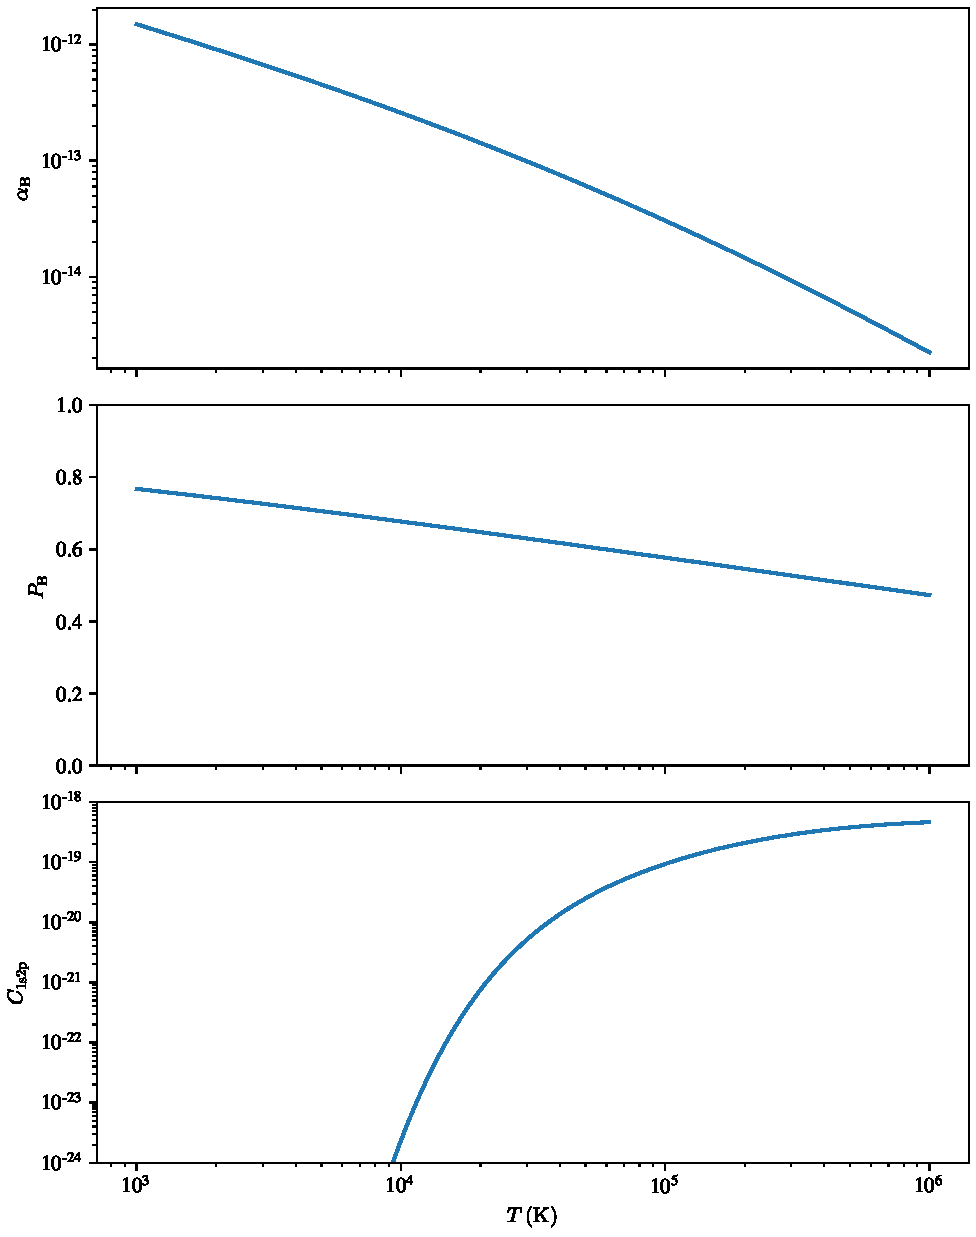
\includegraphics[width=\textwidth,height=\textheight,keepaspectratio]{figures/coefficients.pdf}
  \caption{
      To help explain what impact each of the coefficients in the Ly$\alpha$ rate has, we  plot them here as a function of temperature across the gas temperature range we see the snapshots we have analyzed.
      On top is $\alpha_{\rm{B}}$, the case-B recombination coefficient which
      In the middle is $P_{\rm{B}}$, the probability that a case-B recombination emits a Ly$\alpha$ photon.
      On the bottom is $C_{\rm{1s2p}}$, 
  }
  \label{fig:coefficients}
\end{figure*}

To demonstrate the effective relationship between the sources of Ly$\alpha$ emission and gas physical conditions, in Figure \ref{fig:luminosity_vs_temperature}, we set up a controlled idealized experiment in which we bathe a $1$cm$^{3}$ cube of gas in a radiation field with intensity $J_{\rm UV}$, and plot two limiting cases for the luminosity of this specific volume of gas as a function of temperature: with low $J_{\rm UV}^{\rm min} = 0\ \rm erg\ \rm s^{-1}$ and high $J_{\rm UV}^{\rm max} = 10^{-5}\ \rm erg\ \rm s^{-1}$.
The high-UV value was chosen to fully ionize the gas
\footnote{
    Note that in Figure \ref{fig:luminosity_vs_temperature} we plot the Ly$\alpha$ luminosity across the full temperature range seen in our simulations, but the analytical approximation we use for for $P_B(T)$ only extends out to $10^5$ K because that is the limit of the tables in \citet{Pengelly1964}.
    Therefore we have shaded this region of the plot to indicate that this region where $P_B\left(T\right)$ is being extrapolated from the analytic formulation.
}.

We first consider the $J_{\rm UV}^{\rm min}$ case in Figure~\ref{fig:luminosity_vs_temperature} (purple).
Here, emission is maximized near $T=10^4$ K, because the impact of the gas temperature on collisionally-driven Ly$\alpha$ emission is twofold.
In the very low temperature regime, the ionization rate is sufficiently low that there are no free electrons to collisionally excite the gas.
As the ionization state increases with temperature, there are more free electrons but less neutral hydrogen to be collisionally excited.
However the second effect of temperature is to increase the rate of collisions, which produces a strong mitigating effect against the dropping abundance of neutral hydrogen; even as the gas approaches being fully ionized at high temperatures the rate of collisions mitigates the drop in luminosity.

Turning now to the $J_{\rm UV}^{\rm max}$ case in our idealized numerical experiment (top panel of Figure~\ref{fig:luminosity_vs_temperature}, orange lines) the Ly$\alpha$ emission from recombination declines slowly with temperature.
The $J_{\rm UV}^{\rm max}$ also has a different temperature dependence.
The gas is maximally ionized at all temperatures, but we see a decline in emissivity with temperature because the cross-section of the electrons and hydrogen nuclei drop as their thermal velocities increase, making recombination less likely.
In this experiment, where the the UV field should completely ionize the hydrogen, it is prevented from doing so to preserve numerical stability: the neutral fraction is restricted from dropping below $10^{-10}$.
As a result, in this extreme scenario, the collisional emissivity is driven by this neutral fraction floor, and is therefore unphysical.
Accordingly, we do not plot the collisional emissivity in the $J_{\rm UV}^{\rm max}$ case in Figure~\ref{fig:luminosity_vs_temperature}.

The trends in our controlled experiment (Figure~\ref{fig:luminosity_vs_temperature}) provide us with the physical insight we need to understand which gas in our simulation is emitting Ly$\alpha$, and which gas is not.
In the bottom panel of Figure~\ref{fig:luminosity_vs_temperature}, we show the cumulative distribution of recombination and collisionally-excited emission in a single snapshot.
From this we can see that the bulk of the Ly$\alpha$ photons are produced by ``cold'' photoionized gas gas ($T < 5\times 10^3$ K) and the ``warm'' collisionally-excited gas $(6\times10^3\ \mathrm{K} \leq T \leq 10^4\ \mathrm{K})$.
The emission sources (recombination and collisional de-excitation) are segregated by temperature on account of the astrophysical mechanisms responsible for the gas temperature.
Cooler, recombining gas gas typically lies at high densities with efficient cooling and must be ionized primarily by a nearby UV source, often newly formed stars.

\begin{figure}
  \centering
    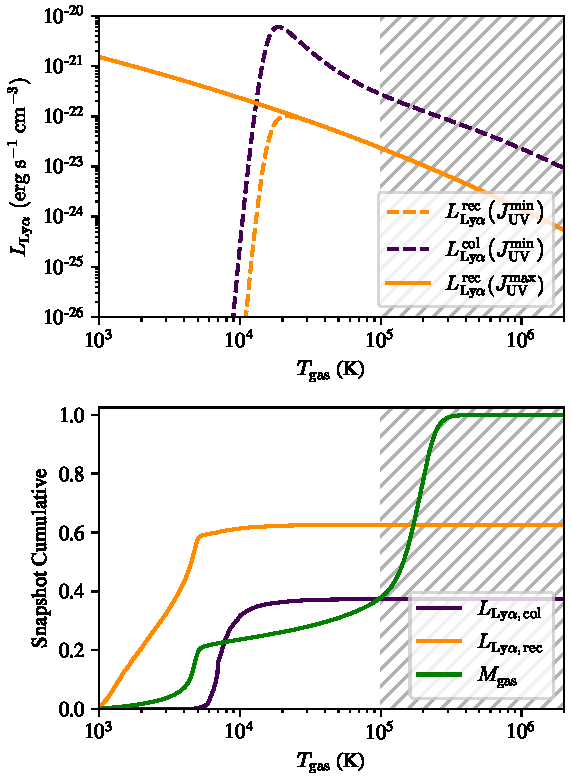
\includegraphics[width=\textwidth,height=\textheight,keepaspectratio]{figures/luminosity_vs_temperature.pdf}
  \caption{
    In the top panel, we show the Ly$\alpha$ luminosity for a parcel of gas typical gas at an average density and metallicity in our simulations as a function of temperature.
    The purple curve represents emissivity as a function of temperature for gas with the minimum ionizing UV field we find in our simulations, and the orange curves are for gas in the strongest ionizing UV field we find.
    The dashed lines represent luminosity due to collisionally excited gas, and the solid lines represent luminosity due to recombinations.
    The gray hatched region for $T > 10^5$ K indicates a temperature range for which we have extrapolated the Ly$\alpha$ conversion probability per recombination event as these probabilities are not computed at $T>10^5$ K in the \citet{Pengelly1964} tables that we utilize.
  }
  \label{fig:luminosity_vs_temperature}
\end{figure}


\section{Ly\texorpdfstring{$\alpha$}{a} Emission from Cosmological Simulations of Massive Galaxy Evolution}

Now that we have built insight into the physics of Ly$\alpha$ emission from collisional excitation and recombination in an idealized experiment, we turn to our galaxy evolution simulations to understand the dominant sources of Ly$\alpha$ luminosity in our model LABs.

In this section, we explore the origin of escaping Ly$\alpha$ in our simulations, where we do not consider the effect of AGN on the ionization state of the gas.
We will discuss the effects of AGN in \S~\ref{sec:agn}.

In Figure \ref{fig:recombination_collision} we plot independently the recombination and collisional excitation components of our fiducial LAB's luminosity.
The contributions from recombination and collisions vary dramatically over the course of the model halo's evolution evolution, though by and large emission from collisionally excited hydrogen dominates, and grows over redshift as this galaxy grows.
Integrating over our redshift of interest ($2 \leq z \leq 5$) we find $\frac{\int L_{\rm Ly \alpha}^{\rm col} dt}{\int L_{\rm Ly \alpha}^{\rm col} + L_{\rm Ly \alpha}^{\rm rec} dt} = 0.80$.
Note, we will \S~\ref{sec:agn} discuss the impact of including an AGN in these models; when we include AGN recombination from emissions dominates and the above ratio becomes $0.03$.

It is tempting to ask whether the dominant power source (recombinations vs collisions) correlated with an obvious physical property of the galaxy?
Across our three galaxies, we do not discover any strong trends (plots of this non-result can be found in Appendix~\ref{app:correlations}).
The reason for this is complex; Ly$\alpha$ emission and escape is complex and we elaborate on this in the following sections.

As we demonstrated in Figure~\ref{fig:luminosity_vs_temperature}, the relative contribution of recombinations and collisions is a complex function of both the gas temperature and incident radiation field on a given parcel of gas.
Galaxies have a large distribution of temperatures and ionization states that vary over the course of their lifetimes, and this distribution does not vary smoothly with a single physical property.
The radiation fields are dependent on the small scale clumping and opacity variations across the galaxy, which result in the dominant power source (recombinations vs collisions) varying non-monotonically across the galaxy.
We see this explicitly in Figure~\ref{fig:121_rec_col}, where we show the morphology of galaxy A4 at redshift $z=3$ while isolating the recombination driven and collisionally driven luminosity, respectively.
The former naturally peaks much more strongly at the center of the galaxy, where star formation normally peaks, which is a source of ionization that is so critical to the rate of recombinations.
However, emission from both physical processes is significant across the bulk of the main disk.

\begin{figure}
    \centering
    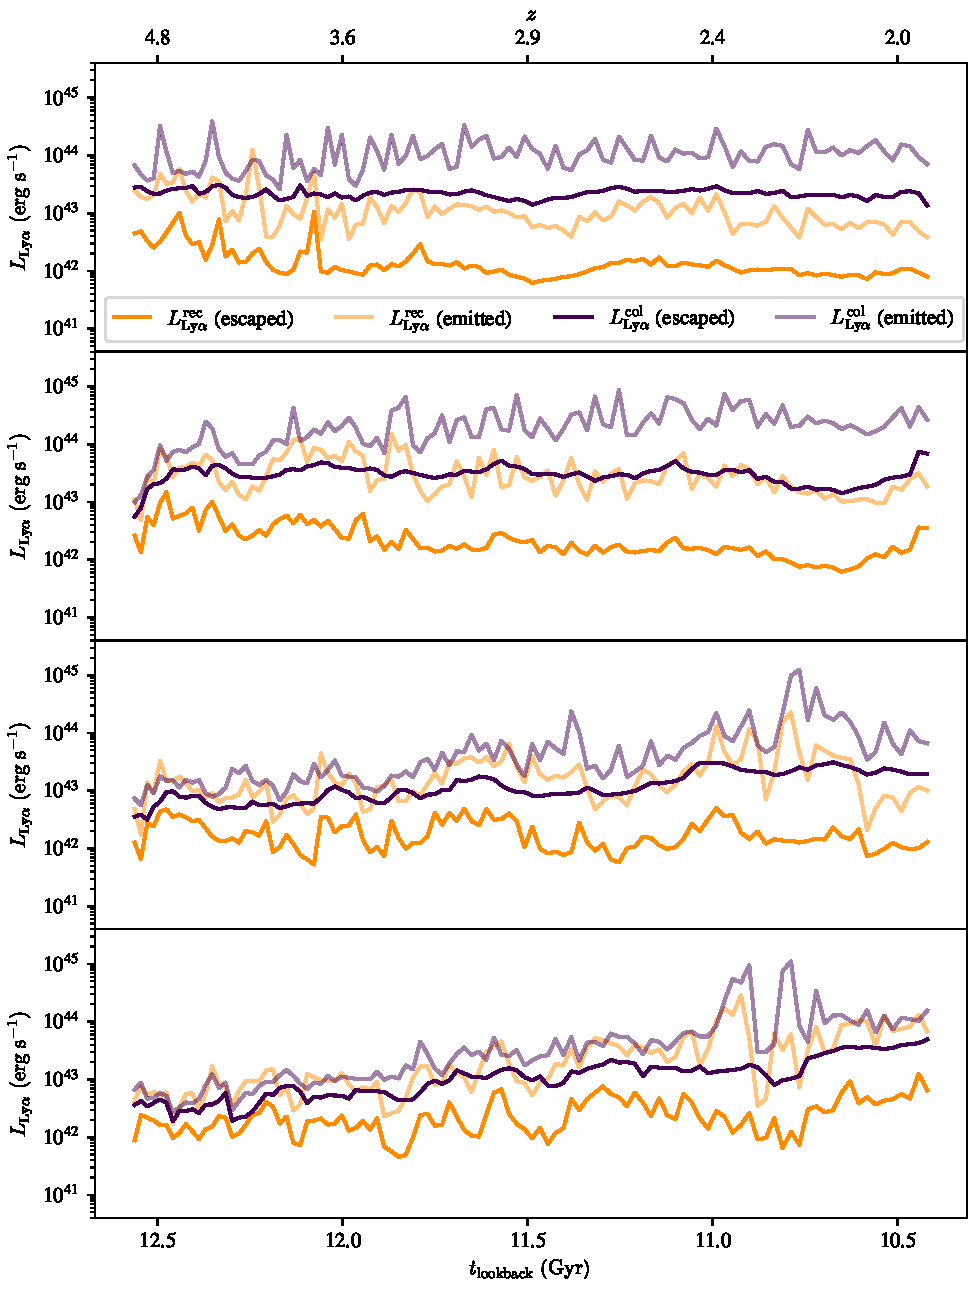
\includegraphics[width=\textwidth,height=0.9\textheight,keepaspectratio]{figures/recombination_collision.pdf}
    \caption{
        We plot the emission of each of our halos due to recombinations and collisions over redshift.
        The darker lines are the luminosity of that component along a median line of sight, the paler lines are that component without accounting for Ly$\alpha$ escape; they can be thought of the intrinsic emission of the halo.
        The distance between the dark and pale lines is the escape fraction of that source at that redshift.
    }
    \label{fig:recombination_collision}
\end{figure}

\begin{figure*}
    \centering
    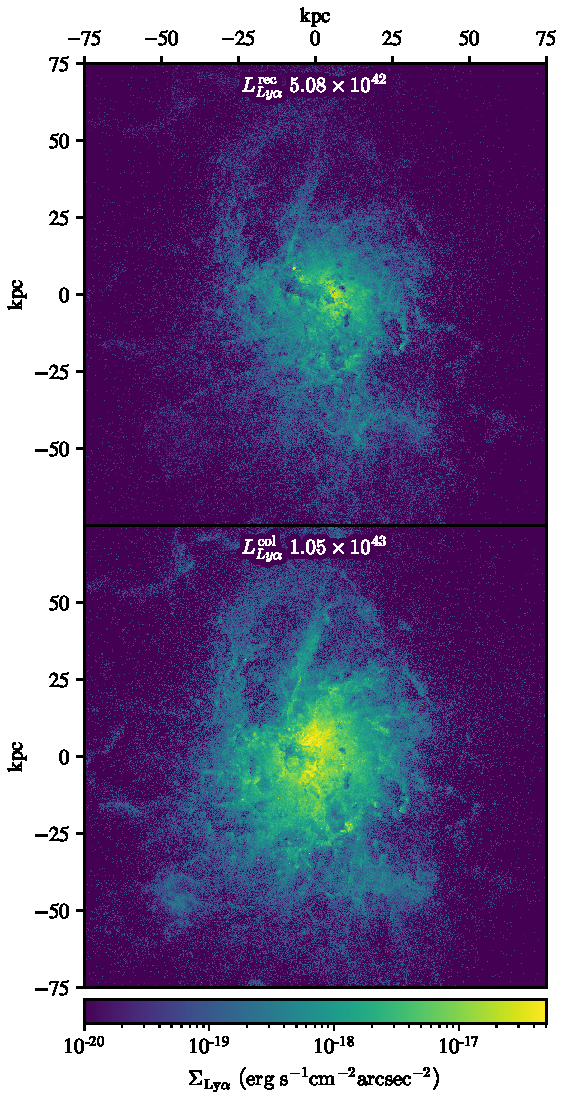
\includegraphics[width=\textwidth,height=0.9\textheight,keepaspectratio]{figures/sb_rec_vs_col.pdf}
    \caption{
        In the top panel is an example surface brightness image produced by running Ly$\alpha$ radiative transfer on a snapshot, taking into account only emission due to recombinations.
        In the bottom panel we only account for emission due to collisional excitation.
        Note that these sources of emission are distributed very differently across the central galaxy; they trace different gas.
    }
    \label{fig:121_rec_col}
\end{figure*}


\section{Impact of the Ionization Post-Processing}

In this project, we had a starting assumption that the on-the-fly ionization state calculations are incorrect enough to alter our results.
One of the great strengths of a computational project like this is that we can perform almost limitless experiments, and so validate such assumptions.

The simplest question towards this direction is whether our ionization state post-processing alters the net ionization state of the simulation.
We plot this difference in \ref{fig:pre_post_ionization}, demonstrating that there is some effect on the gas state due to our post-processing.
But does this change in the ionization state alter the Ly$\alpha$ properties of the simulation?
The ionization state is important to the luminosity of Ly$\alpha$ and to its escape properties, but there is a lot of complexity in these simulations, most notably that population of high-temperature gas seen in Figure~\ref{fig:121_rec_col}.
It is possible that we have only recomputed the state of gas that does not significantly participate in Ly$\alpha$ radiative transfer.
% TODO: Make this figure
% In \ref{fig:pre_post_escape} we plot the intrinsic Ly$\alpha$ luminosity and escape fraction for our halos when we do not do any ionization state post-processing.
It would be educational to perform an experiment to test this hypothesis.


\begin{figure}
    \centering
    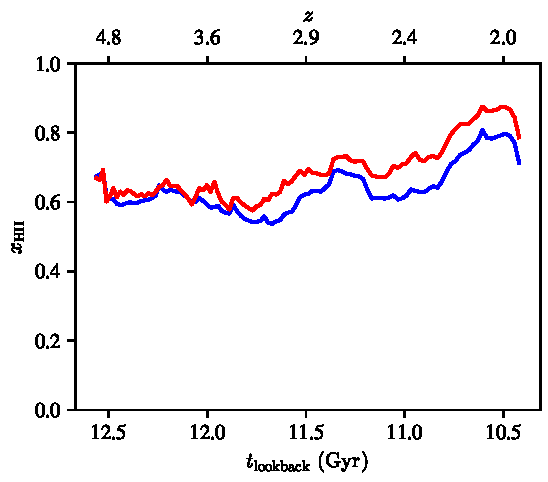
\includegraphics[width=\textwidth,keepaspectratio]{figures/ionization_state.pdf}
    \caption{
        We plot the mass-weighted ionization state of the simulation domain we use in this work over redshift, in blue is the ionization state we get directly from a snapshot, and in red is the ionization state we compute ourselves using collisional equilibrium and ionizing radiative transfer.
        Our post-processed ionization state is significantly elevated, and is more and more discrepant at lower redshifts.
    }
    \label{fig:pre_post_ionization}
\end{figure}


\section{The Impact of Stars}

In the preceeding sections, we have often referred to stars as a driver of ionization.
For the most part in astronomy, this is common sense.
Short-lived high-mass stars emit very strongly at wavelengths that are sufficient to ionize hydrogen and because of the long legacy of studying stars, have a sort of subconscious association in the field.
One would reasonably assume that some gas is ionized, so there must be a lot of young stars.
But as ever in this work we are running computer simulations and thus we can control physics and otherwise rearrange the universe to our liking.
We can replace an assumption with an experiment.

In Figure~\ref{fig:stars} we plot the intrinsic and escaping luminosity with and without the presence of stars in our post-processing ionization state calculation.
The addition of stars increases the intrinsic Ly$\alpha$ emission in the simulation, but rarely by a factor of 2 or more.
By contract, the escaping Ly$\alpha$ is hardly changed at all by the addition of stars to the ionization state calculation.

Our conclusion from this observation is \emph{not} that star formation does not impact the luminosity and/or escape fraction of Ly$\alpha$ from massive galaxies.
The ionization state post-processing that we do cannot and does not compute the ionization state of the gas entirely on its own.
As ever, the critical input to this system is the temperature of the gas.
Recall that we are taking the gas temperature directly from the FIRE-2 zoom simulations, and we do not attempt to update it to reflect our inputs or in this case, the lack of an input.
These temperatures we get from FIRE-2 already contain the influence of stars, the information for which is contained in both the gas temperature and ionization state.
These two properties are part of an equilibrium, and in removing the stars from our ionization state calculations we have effectively perturbed one part of this system and caused it to relax into a different state.

\begin{figure}
    \centering
    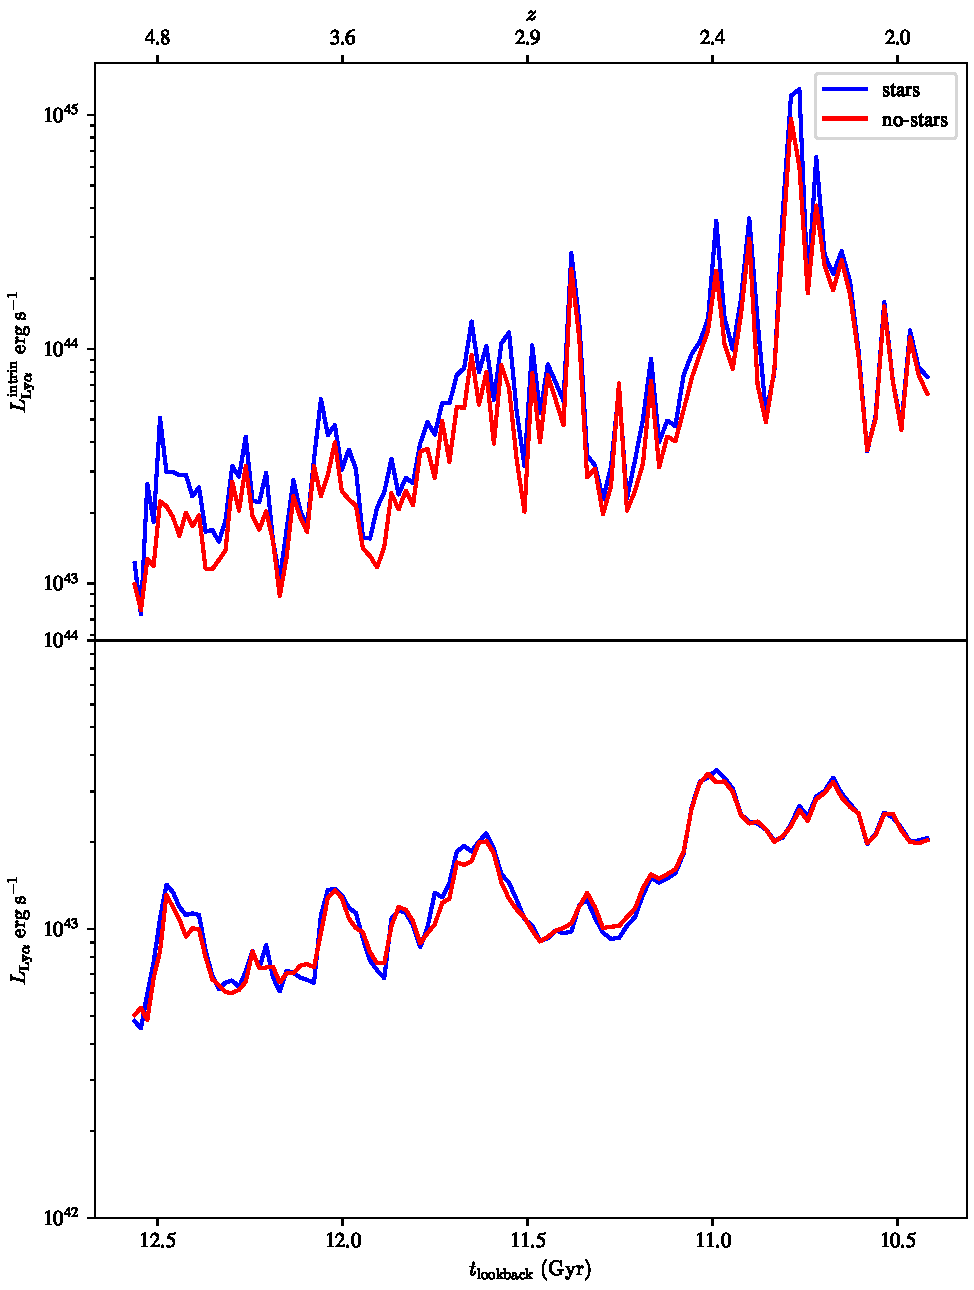
\includegraphics[width=\textwidth,height=0.85\textheight,keepaspectratio]{figures/stars.pdf}
    \caption{
        In the top panel, we plot the intrinsic Ly$\alpha$ luminosity of a halo with and without ionizing radiation from stars accounted for in the ionization state calculation step.
        In the bottom panel, we plot the escaping Ly$\alpha$ luminosity along a median line of sight for the same halo.
        While the presence of stars does increase the amount of Ly$\alpha$ emitted by the halo gas, this change is much less substantial when we account for the physics of Ly$\alpha$ escape.
    }
    \label{fig:stars}
\end{figure}


\section{Line-Of-Sight Dependence}
\label{sec:los}

Often in this work we will plot or discuss the Ly$\alpha$ luminosity of a halo for a median line of sight.
This deserves explanation on two accounts; the choice of median and the importance of line of sight in general.

We choose the median because in almost all discussion of the Ly$\alpha$ luminosity of a halo, we are trying to make some connection to either the range of observed luminosities as in Figure~\ref{fig:luminosity_redshift}, or we want a single value to simplify our data visualization.
The median of the distribution is notionally the most likely value to observe if the object is randomly placed on the sky, wheras the mean luminosity may be strongly biased by lines of sight with particularly high escape fractions, and therefore particularly high observed Ly$\alpha$ luminosity.

Such lines of sight can arise from an ionized region embedded asymmetrically in a cloud of neutral hydrogen.
In the limit where an ionization front breaks through the cloud of neutral hydrogen, this geometry comes to resemble a laser cavity.
A large amount of Ly$\alpha$ is emitted within the ionized region but when a photon scatters off material near the interface, a random step in the direction of greater optical depth is more likely to be short than a random step in the direction of lower optical depth which is away from the neutral hydrogen.
Because of this interaction an interface between ionized and neutral hydrogen is almost reflective to Ly$\alpha$.
From basic intiution, it does not seem like a cloud of gas would be asymmetric in brightness by more than an order of magnitude, but it is not far from the truth to think of these systems as composed of large semi-reflective surfaces.
Of course the system is more complex than this thought experiment because all the gas in the system will emit in Ly$\alpha$, to varying degrees.

We are able to calculate Ly$\alpha$ escape fraction over many lines of sight because we can compute it using only the direction and position of Ly$\alpha$ photons when they exit the simulation domain.
To compute the escape fraction over some arbitrary line of sight, we select photons that escape approximately towards that direction, weight them according to the angle between their direction and the desired line of sight, and compute the sum of their escaping weights over the sum of their emitted weights.

\begin{figure}
    \centering
    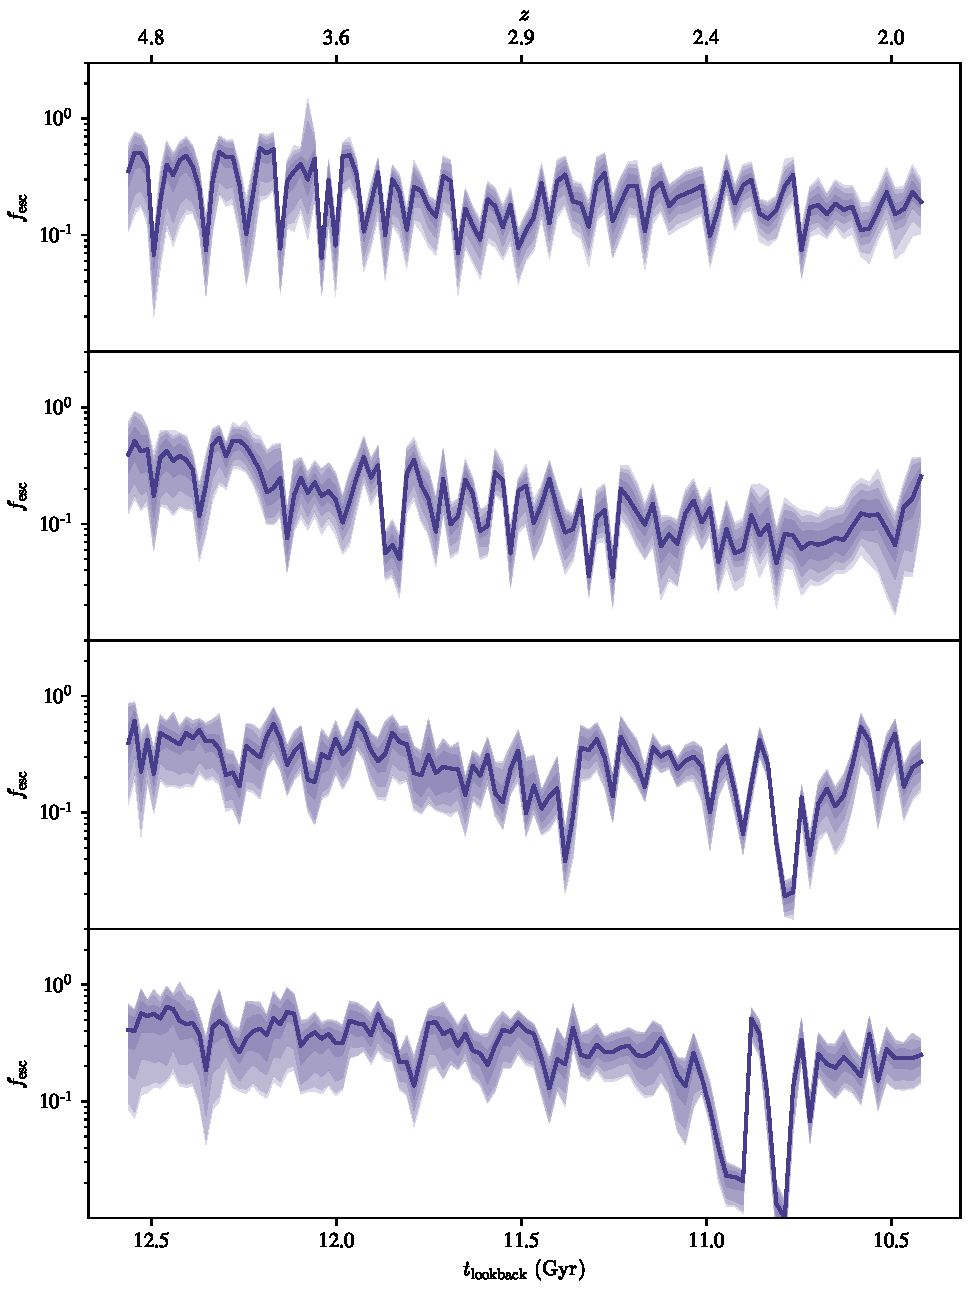
\includegraphics[width=\textwidth,height=0.85\textheight,keepaspectratio]{figures/los.pdf}
    \caption{
        We plot the escape fraction from each of our halos over redshift, and in the shaded regions around the central dark line show the 1-$\sigma$, 2-$\sigma$, and 3-$\sigma$ extent of the distribution as well as the min and max in the palest color.
        These escape fractions were calculated at each redshift over 3072 evenly-spaced angles.
    }
    \label{fig:los}
\end{figure}
